The Input/Output layer is a client-side interface for the user to visualize the output of the drone detection and communicate with the drone detection system. The Input/Output layer has three subsystems: Results Display, User Inputs and Application.

\subsection{Results Page}
The results page includes the output of the drones detected in the area which is presented to the user in graphical form. 


\begin{figure}[h!]
	\centering
 	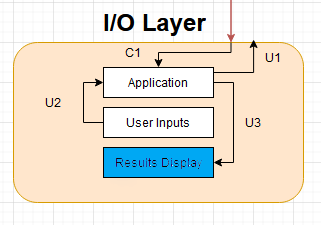
\includegraphics[width=0.60\textwidth]{images/results.png}
 \caption{Results Display Subsystem Diagram}
\end{figure}

\subsubsection{Assumptions}
The results page will only be online after the system is turned on.

\subsubsection{Responsibilities}
The responsibility of the results page is to communicate with the database through the application interface to provide the graphical visualization of the location of the system and any drones detected in the surrounding area. The results page will display the location of the device in the form of circular dot and any detected drones will be shown in triangular shape.

\subsubsection{Results Subsystem Interfaces}

\begin {table}[H]
\caption {Results interfaces} 
\begin{center}
    \begin{tabular}{ | p{1cm} | p{5cm} | p{4cm} | p{4cm} |}
    \hline
    ID & Description & Inputs & Outputs \\ \hline
    \#U3 & Communication with application & \pbox{4cm}{detected drones and system location data from the database} & \pbox{4cm}{Graphical view of the detected drones and location of the system}  \\ \hline
   
    \end{tabular}
\end{center}
\end{table}

\subsection{User Inputs}
The User Inputs page includes the input that can be taken from the user. Here, the user can select a detected drone and verify that it is a false positive. Also, user can select an individual drone and the system will actively track the selected drone in as close to real time as possible.


\begin{figure}[h!]
	\centering
 	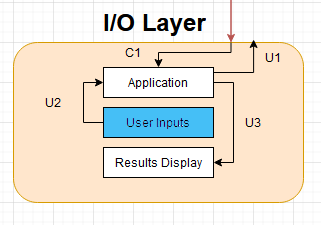
\includegraphics[width=0.60\textwidth]{images/userInputs.png}
 \caption{User Inputs subsystem diagram}
\end{figure}

\subsubsection{Assumptions}
The user can only select one drone at a time for active detection.

\subsubsection{Responsibilities}
The responsibility of the User Inputs is to provide a user interface to the user where they can select a detected drone and verify that it is a false positive. Also, the user can select an individual drone and the system will actively track the selected drone in as close to real time as possible.

\subsubsection{User Inputs Subsystem Interfaces}

\begin {table}[H]
\caption {User Inputs Subsystem interfaces} 
\begin{center}
    \begin{tabular}{ | p{1cm} | p{5cm} | p{5cm} | p{5cm} |}
    \hline
    ID & Description & Inputs & Outputs \\ \hline
    \#U201 & Single Drone Active Tracking & \pbox{5cm}{Select input from the user} & \pbox{5cm}{Selected Drone highlighted and actively tracked}  \\ \hline
    \#U202 & False Positive in detected Drones  & \pbox{5cm}{Select input from the user} & \pbox{5cm}{The selected object will not be further tracked}  \\ \hline
    \end{tabular}
\end{center}
\end{table}

\subsection{Application Subsystem}



\begin{figure}[h!]
	\centering
 	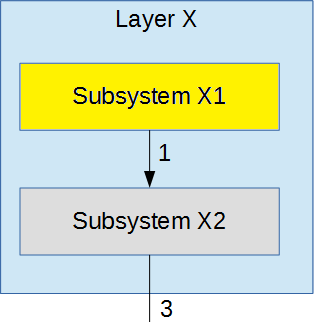
\includegraphics[width=0.60\textwidth]{images/subsystem.png}
 \caption{Example subsystem description diagram}
\end{figure}

\subsubsection{Assumptions}


\subsubsection{Responsibilities}


\subsubsection{Subsystem Interfaces}

\begin {table}[H]
\caption {Subsystem interfaces} 
\begin{center}
    \begin{tabular}{ | p{1cm} | p{6cm} | p{3cm} | p{3cm} |}
    \hline
    ID & Description & Inputs & Outputs \\ \hline
    \#01 & Description of the interface/bus & \pbox{3cm}{input 1 \\ input 2} & \pbox{3cm}{output 1}  \\ \hline
    \#xx & Description of the interface/bus & \pbox{3cm}{N/A} & \pbox{3cm}{output 1}  \\ \hline
    \end{tabular}
\end{center}
\end{table}


